\hypertarget{technical-survey}{%
\chapter{Technical Survey}\label{technical-survey}}

In this chapter we will perform a high level survey of the available
tools and approaches that could be used for \gls{e3} and select ones
that fit our requirements. In the next chapter we will go more in depth
and cover the implementation details using those tools.

Since we need to design for a heterogeneous runtime environment, we need
to choose building blocks that are compatible with as many scenarios as
possible while also keeping the complexity low.

\hypertarget{deployment}{%
\section{Deployment}\label{deployment}}

Our primary users are enterprises and power users. Enterprises can
employ a variety of \gls{iac} tools in their infrastructure management
process:

\begin{itemize}
\tightlist
\item
  provisioning - Terraform\autocite{tfDocs}, Cloud
  Formation\autocite{cfDocs}, etc.
\item
  deployment automation - Ansible\autocite{ansibleDocs},
  Puppet\autocite{puppetDocs}, Chef\autocite{chefDocs}, etc.
\item
  container orchestration - Docker Swarm\autocite{dockerDocs},
  Kubernetes\autocite{kubeDocs}, etc.
\end{itemize}

According to our definitions, power users typically use physical
machines while enterprises can use both virtual machines and container
orchestration tools. Based on our requirements for \gls{e3} we need a
cross region deployment. \glspl{vm} can be automatically provisioned
across different regions in the cloud using \gls{iac} tools. Once
provisioned, a \gls{vm} is usually managed via an automation tool that
executes a set of deployment steps over SSH. Those deployment steps can
be adapted to physical machines so that power users can make use of
them.

Kubernetes is used for dynamically scaling a large number of
long-running processes across a cluster of \glspl{vm} within the same
geographic region. Enterprises may wish to run MPyC programs in a
Kubernetes cluster and might benefit from an example of doing so. But
for the purposes of \gls{e3}, it does not provide sufficient benefits
compared to using \glspl{vm} directly, while it adds complexity in terms
of deploying multiple clusters across regions and adding a cross cluster
communication mechanism.

Based on this analysis, we choose to base \gls{e3} on a combination of
\glspl{vm} deployed in the cloud and a set of personal devices owned by
the authors - a Linux laptop, a Windows desktop with Windows Subsystem
for Linux, and an ARM Raspberry Pi 2 to serve as an example of both
enterprises and individual power users.

\gls{iac} tools use specifications that are either imperative or
declarative. \textbf{Imperative} specifications describe the steps
needed to be executed for the infrastructure to reach the desired state,
while \textbf{declarative} specifications describe the desired final
state and let the tool worry about how to get there. Imperative tools
are more likely to suffer from \emph{configuration drift} - the
infrastructure state might become out of sync with the specification due
to either manual changes or left-over state from previously applied
specifications. On the other hand, if something is removed from a
declarative specification, when it gets applied, the corresponding
resources will also be removed from the infrastructure. In addition,
declarative tools are idempotent - applying the same specification
multiple times in a row does not change the state. Therefore in order to
achieve high reproducibility, we will prefer declarative tools to
imperative ones where possible.

On Linux, software is usually installed via package managers. Most of
the popular Linux distributions such as Ubuntu, Debian, Fedora, Arch use
package managers that only support automating this process via
imperative shell scripts rather than a declarative specification.
Additionally those do not offer an easy way of specifying and locking
the required software versions to a known good configuration that can be
reproduced in the future. NixOS on the other hand is based on the
declarative Nix package manager which does support version locking via
its \textbf{flakes} feature. This is why we choose to use the NixOS
operating system for our \glspl{vm}.

Most of the popular application deployment tools such as Ansible, Chef
and Puppet are either imperative or have limited support for declarative
specifications. Fortunately, the NixOS ecosystem, offers a number of
deployment tools that can apply a declarative specification on remote
hosts:

\begin{itemize}
\tightlist
\item
  NixOps\autocite{nixopsSource,nixopsDocs} - official tool
\item
  Colmena \autocite{colmenaSource,colmenaDocs}
\item
  morph \autocite{morphSource}
\item
  deploy-rs \autocite{deployrsSource}
\end{itemize}

NixOps is the official deployment tool for NixOS but it was being
redesigned at the time of writing. The new version was not complete yet
and lacked documentation, while the old one was no longer being
supported and depended on a deprecated version of Python. The rest of
the tools were still actively maintained. Colmena was the best fit for
our use case because it supported both flakes and parallel deploys,
while morph lacked support for flakes and deploy-rs could not deploy to
multiple hosts in parallel.

The declarative tools that were considered for provisioning were
Terraform, Pulumi and Cloud Formation. Cloud Formation only works on AWS
which would prevent us from using it with other cloud providers. Pulumi
is a newer and less proven tool compared to Terraform, which the authors
had more experience with. Therefore our choice was to use Terraform.

We decided to use DigitalOcean as a cloud provider because they are
supported by Terraform and offered free credits for educational use.

\hypertarget{connectivity}{%
\section{Connectivity}\label{connectivity}}

There are a number of approaches for communication between our host
machines. During the preparation phase of the project we will perform a
high level exploration of our options and summarize them. For \gls{e3}
we will initially use the simplest to implement one. During the
implementation phase of the project we will go more in depth and
implement more approaches and analyze how they compare to each other in
practice.

\hypertarget{virtual-private-networks-vpns}{%
\subsection{Virtual Private Networks
(VPNs)}\label{virtual-private-networks-vpns}}

\glspl{vpn} are commonly used for securely connecting machines from
different \glspl{lan}. They provide software emulation of a network
device on the operating system level and allow other software to
transparently use the functionality of the \gls{ip} suite without
requiring extra changes. Traditional \glspl{vpn} such as
OpenVPN\autocite{openVPNDocs} use a centralized service that all
(encrypted) client communications must pass through. This introduces a
single point of failure and a potential bottleneck that might negatively
impact the performance of the multi-party computations due to their
\gls{p2p} nature.

\begin{figure}
\centering
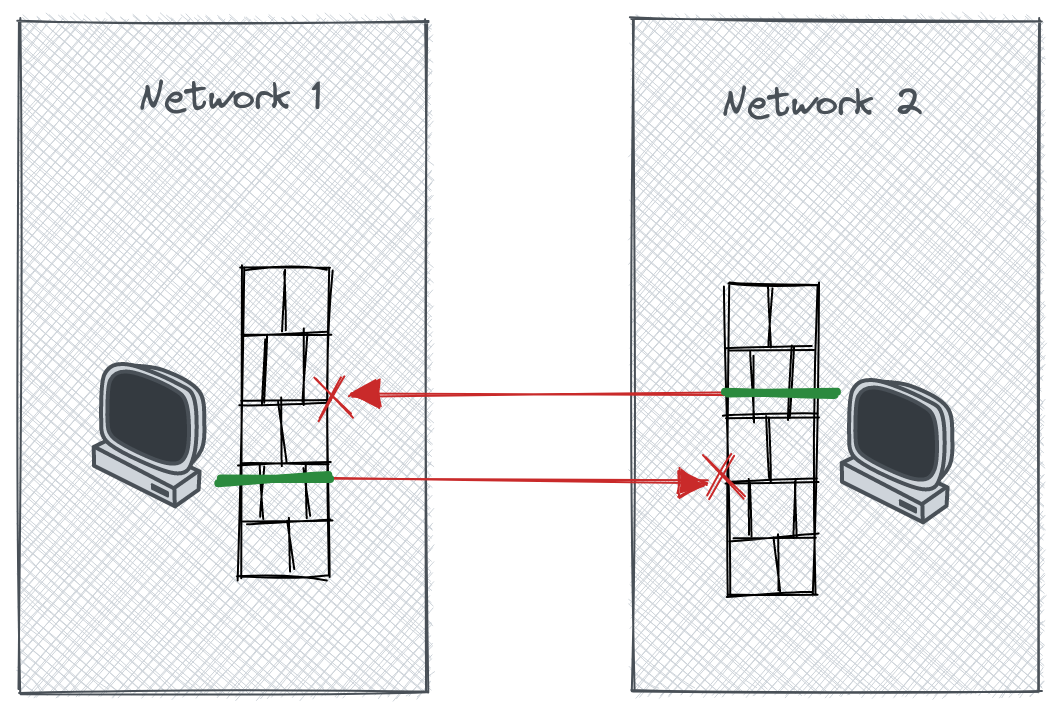
\includegraphics[width=0.5\textwidth,height=0.25\textheight]{prep/../figures/nat-intro.png}
\caption{``Two parties behind separate NATs''\label{nat-intro}}
\end{figure}

On the other hand, mesh \glspl{vpn} such as Tinc\autocite{tincDocs},
Tailscale\autocite{tailscaleDocs} and Nebula\autocite{nebulaDocs}
utilize direct \gls{p2p} links between the clients for the data traffic.
Authentication, authorization and traffic encryption are performed using
certificates based on public key cryptography. As we mentioned in the
introduction chapter, the devices in a typical home network can only
initiate connections to public endpoints (via \gls{nat}) but cannot be
discovered from outside their \gls{lan}. This poses a challenge when two
parties who want to communicate via a direct link are both behind
separate \glspl{nat} \ref{nat-intro} and neither can be contacted by the
other one first. Mesh \glspl{vpn} solve this issue via \gls{nat}
traversal techniques such as \gls{udp} hole punching based on concepts
from \gls{stun}. The machines of each party can contact a public
\gls{stun} server \ref{nat-traversal}, which will note what \gls{ip}
addresses the connections come from and inform the parties. Since the
parties initiated the connection to the STUN server, their routers will
keep a mapping between their local IP addresses and the port that was
allocated for the connection in order to be able to forward the incoming
traffic. Those ``holes'' in the NATs were originally intended for the
STUN server, but mesh VPNs use the stateless ``fire and forget'' UDP
protocol for their internal communication, which does not require nor
provides a mechanism for the NATs to verify who sent a UDP packet. With
most NATs, this is enough to be able to (ab)use the ``punched holes''
for the purpose of \gls{p2p} traffic from other parties. Mesh VPNs
implement the stateful \gls{tcp} and \gls{tls} protocols on top of UDP
and expose an regular network interface to the other programs, keeping
them shielded from the underlying complexities. Other NAT
implementations such as Symmetric NAT and \glspl{cgnat} can be more
difficult to ``punch through'' due to their more complex port mapping
strategies. In those cases, establishing P2P connections might involve
guess work or even fail and require falling back to routing the
(encrypted) traffic via another party or service.

\begin{figure}
\centering
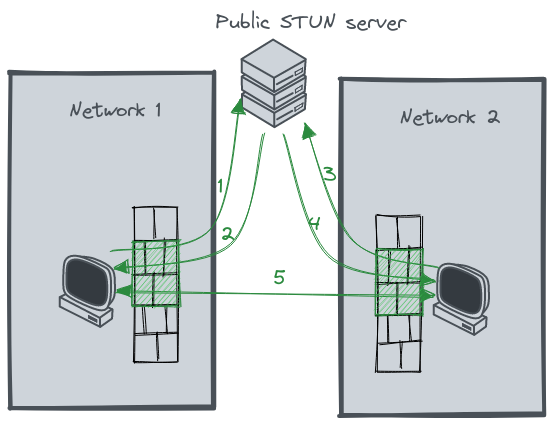
\includegraphics[width=0.5\textwidth,height=0.25\textheight]{prep/../figures/nat-traversal.png}
\caption{``NAT traversal via STUN''\label{nat-traversal}}
\end{figure}

Now that we have a general understanding of how mesh VPNs work, let us
see how Tinc, Tailscale and Nebula compare. All three are open-source,
with the exception of Tailscale's coordination service which handles the
peer discovery and identity management. Headscale
\autocite{fontJuanfontHeadscale2022} is a community driven open-source
alternative for that component. Tinc is the oldest of the three but has
a relatively small community. It is mainly developed by a single author
and appears to be more academic than industry motivated. Nebula and
Tailscale are both business driven. Tailscale was started by a number of
high profile ex-googlers and is the most end-user focused of the three,
providing a service that allows people to sign up using a variety of
identity providers including google, microsoft, github and others. They
also provide an Admin console that allows a user to easily add their
personal devices to a network or share them with others. It also has
support for automation tools like Terraform for creating authorization
keys and managing an \gls{acl} based firewall. Nebula was originally
developed at the instant messaging company Slack to create overlay
networks for their cross region cloud infrastructure, but the authors
later started a new company and are currently developing a user-centric
platform similar to Tailscale's. Nebula is more customizable than
Tailscale and since it is completely open-source it can be adapted to
different use cases, but it is also more involved to set up. A
certificate authority needs to be configured for issuing the identities
of the participating hosts. Furthermore, publicly accessible
coordination servers need to be deployed to facilitate the host
discovery. Tailscale employs a distributed relay network of \gls{derp}
servers, while Nebula can be configured to route via one of the other
peers in the VPN.

We decided to use Tailscale for the initial implementation of \gls{e3}
because it has all the necessary features to support networked MPC while
also being the easiest one to set up as it does not require any extra
services to be deployed.

We will now briefly mention some additional approaches we looked into
that may be a good starting point for the next phase of the project.

\hypertarget{decentralized-identifiers-dids-and-didcomm}{%
\subsection{Decentralized Identifiers (DIDs) and
DIDComm}\label{decentralized-identifiers-dids-and-didcomm}}

\gls{ssi} is a way of managing a digital identity that emphasises an
individual's ownerhip and control over their personal data. In contrast
with more traditional methods, SSI does not rely on a third party such
as a government or an organization to issue identities - people issue
their own identities, usually in the form of an asymmetric key-pair.
\glspl{did}\autocite{didW3C} are a form of \gls{ssi} that recently
reached W3C Recommendation Status and DIDComm\autocite{didcommSpec} is a
set of communication protocols based on DIDs. Its main design goals are
to be private, secure, decentralized, transport agnostic and routable.
Its primary concerns are with the message formats, cryptograhic
algorithms and processes that enable identity owners to find each other
and interact digitally based on their identities rather than TCP
concepts like IP addresses. One thing we noticed was that the initial
version of DIDComm does not support stateful sessions and therefore all
messages need to be both encrypted with the recepient's public key and
signed by the sender's private key. This will likely cause performance
issues in the MPC setting because it usually involves a large number of
small messages containing the secret shares of the parties. In order for
DIDComm to be usable for MPyC we would likely have to implement a
TLS-like protocol on top of it that supports sessions.

\hypertarget{the-onion-router-tor}{%
\subsection{The Onion Router (TOR)}\label{the-onion-router-tor}}

Two machines need to know each other's IP addresses in order to be able
to interact via the internet. An IP address can reveal details about a
person's location or be used to launch a \gls{ddos} attack against them.
Additionally, nearby attackers could be listening to their traffic and
tracking their internet behaviour, which may be undesirable depending on
a person's privacy requirements. TOR uses a network of relays to
obfuscate the communication route between two parties. The original
sender prepares a multi-layered message, where each layer is encrypted
for a specific relayer. When one of them receives a message, they only
know who was the previous link and after decrypting their part of the
message, they know the next link. They do not know who was the original
sender and who is the final destination. The privacy comes at the cost
of performance. Additionally, TOR has the concept of Onion Services,
which receive an address under the .onion pseudo top level domain and
correspond to a public key
(e.g.~vww6ybal4bd7szmgncyruucpgfkqahzddi37ktceo3ah7ngmcopnpyyd.onion).
It allows two way privacy preserving communications. A concept similar
to TOR can be optionally incorporated in MPyC for the cases when privacy
is essential. It is interesting to measure the performance impact on
MPyC computations when routed via a TOR-like relay network.

\hypertarget{summary}{%
\section{Summary}\label{summary}}

In this chapter we compared a number of potential building blocks for
\gls{e3} and made some choices informed by our requirements.
Specifically, we will use Terraform for provisioning Virtual Machines
running NixOS on DigitalOcean and Colmena for deploying to them. Our
initial implementation will use Tailscale as the connectivity layer due
to its ease of use. In the next phase of the project, we plan to explore
solutions based on Nebula, DIDComm, TOR and combinations of the above.
